%%This is a very basic article template.
%%There is just one section and two subsections.
\documentclass[12pt,a4paper]{article}
\usepackage{ucs}
\usepackage[T2A]{fontenc}
\usepackage[utf8]{inputenc}
\usepackage[english,bulgarian]{babel}
%\usepackage[margin=1in]{geometry}
\usepackage{listings}
\usepackage{color}
\usepackage{textcomp}
\usepackage[framed]{mcode}
\usepackage{graphicx}
\usepackage{caption}
\usepackage{subcaption}

\addto\captionsbulgarian{%
  \renewcommand{\contentsname}%
    {Содржина}%
  \renewcommand{\tablename}%
    {Табела}%
  \renewcommand{\figurename}%
    {Слика}%
  \renewcommand{\bibname}%
    {Библиографија}%
  \renewcommand{\listfigurename}%
    {Листа на слики}%
  \renewcommand{\listtablename}%
    {Листа на табели}%
}
\renewcommand\lstlistingname{Код фрагмент}


\begin{document}

\title{Имплементација на алгоритми од машинско учење во Matlab/Octave}

\author{Томче Делев}
\date{}

\maketitle

\section{Вовед}

Машинско учење е подобласт на вештачката интелигенција. Со помош на алгоритми
таа се обидува да извлече што е можно повеќе корист од компјутерите кои
претставуваат најмоќни пресметковни машини. Примери на машинско учење се
рударењете на податоци од огромни бази на податоци, медицински записи, биолошки
податочни множества, како и ефикасното пребарување на веб. Голема примена наоѓа
и во области како обработка на природни јазици, препознавање на ракопис,
компјутерска визија итн.

Алгоритмите за машинско учење се подделени во две категории:
\begin{itemize}
  \item надгледувано учење,
  \item ненадгледувано учење.
\end{itemize}
Други видови на машинско учење вклучуваат засилено учење и системи за
препорачување.

Според резултатот од алгоритмот за машинско учење разликуваме алгоритми за
регресија и алгоритми за класификација. Во алгоритмите за регресија се
предвидува континуална променлива, додека во алгоритмите за класификација се
одредува класата (дискретна вредност) на примерокот кој се класифицира.


\section{Линеарна регресија}

\subsection{Линеарна регресија со една променлива}
Ова е имплементација на алгоритам за линеарна регресија кој го предвидува
профитот на камион кој превезува храна. Да предпоставиме дека вие сте извршен
директор на ланец ресторани и сакате да го проширите вашиот ланец во некој
друг град. Во ланецот веќе имате камиони во многу различни градови и имате
податоци за профитот и популацијата во тие градови. 

Сакате со помош на овие податоци да добиете помош кој да биде следниот ваш град
во кој ќе се проширите.

Во датотеката population\_profit.txt се наоѓа податочното множество за проблемот
на линеарна регресија. Во првата колона е популацијата на градот, а во втората е
профитот на камионот во тој град. Негативна вредност на профитот значи загуба.

\subsubsection{Исцртување на податоците}

Пред да се започне со било која обработка, вообичаено е корисно да се разберат
податоците со помош на визуелизација. За да ги визуелизираме овие податоци
користиме scatter plot, поради тоа што има само две својства кои се прикажуваат
(профит и популација).


\lstinputlisting[firstline=6,lastline=8,caption=Вчитување на податоците во променливите $X$ и $y$.
]{src/linearRegression.m}


\lstinputlisting[firstline=6,lastline=10,caption=Исцртување на податоците]{src/plotData.m}


\begin{figure}[htb]
\centering
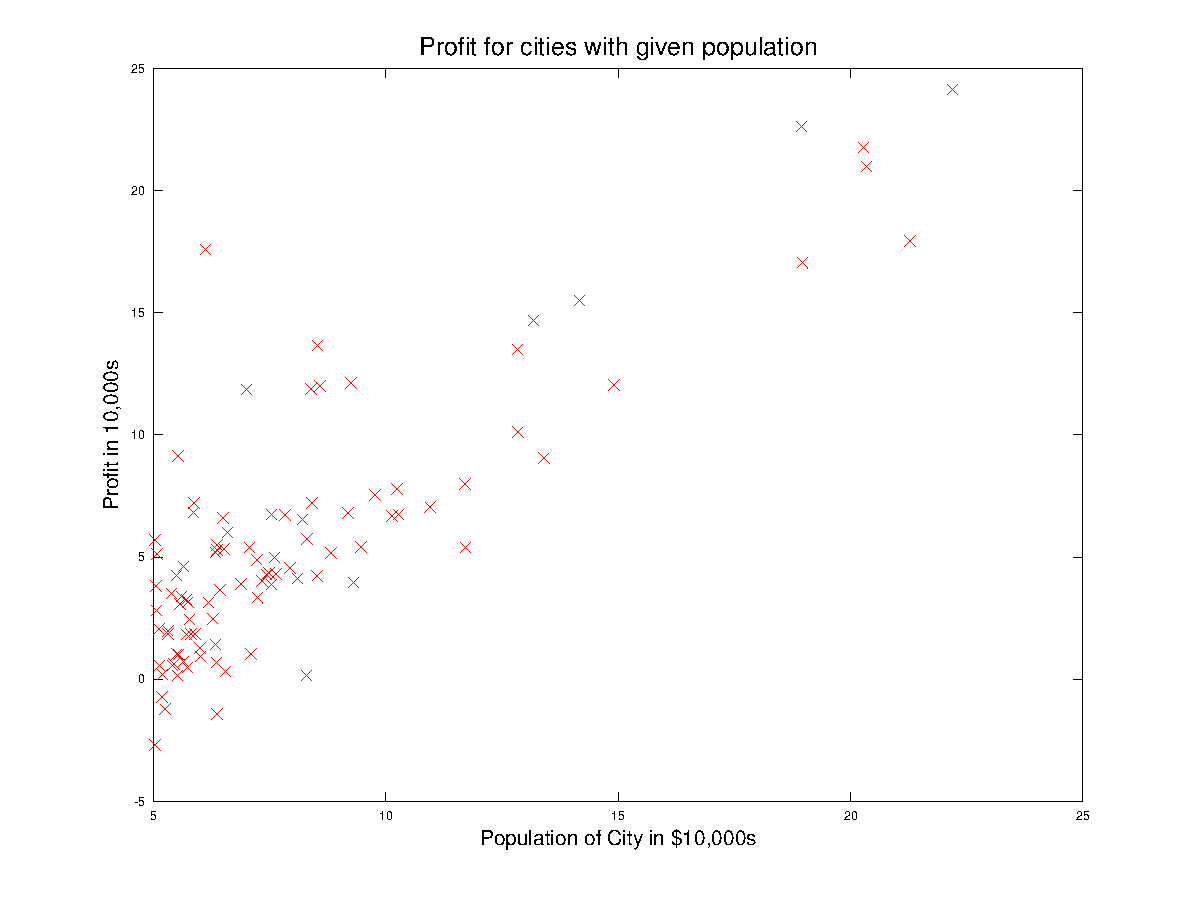
\includegraphics[width=.9\textwidth]{src/data}
\caption{Scatter plot на податочното множество}
\label{fig:plot}
\end{figure}

\subsubsection{Пресметување со Gradient Descent}

Следува имплементација на одредување на параметарот $\theta$ од лиенарната
регресија на податочното множество со помош на gradient descent.

\subsubsection{Равенки за пресметување}

Целта на линеарната регресија е да ја минимизира функцијата на чинење

\[
	J(\theta) = \frac{1}{2m}\sum{(h_\theta(x^{(i)}) - y^{(i)})^2}
\]
каде што хипотезата $h_\theta(x)$ е дадена со линеарниот модел:
\[
	h_\theta(x) = \theta^Tx = \theta_0 + \theta_1x_1
\]

Параметрите на моделот се вредностите $\theta_j$.
Алгоритмот го имплементираме со тоа што во секоја итерација ја извршуваме
следата формула:
\[
	\theta_j := \theta_j - \alpha\frac{1}{m}\sum{(h_\theta(x^{(i)}) - y^{(i)}) x_j}
\]
\emph{Симултано ги менуваме вредностите на $\theta_j$ за секое $j$.}

\subsubsection{Имплементација}

\lstinputlisting[firstline=23,lastline=28,caption=Додавање на дополнителна
колона $\theta_0$ и иницијализција на параметрите.]{src/linearRegression.m}

\subsubsection{Пресметување на функцијата на чинење $J(\theta)$}

\lstinputlisting[firstline=6,lastline=12,caption=Имплементација на
$J(\theta)$]{src/computeCost.m}

\subsubsection{Gradient Descent}

\lstinputlisting[firstline=6,lastline=16,caption=Имплементација
на Gradient Descent]{src/gradientDescent.m}

\begin{figure}[htb]
\centering
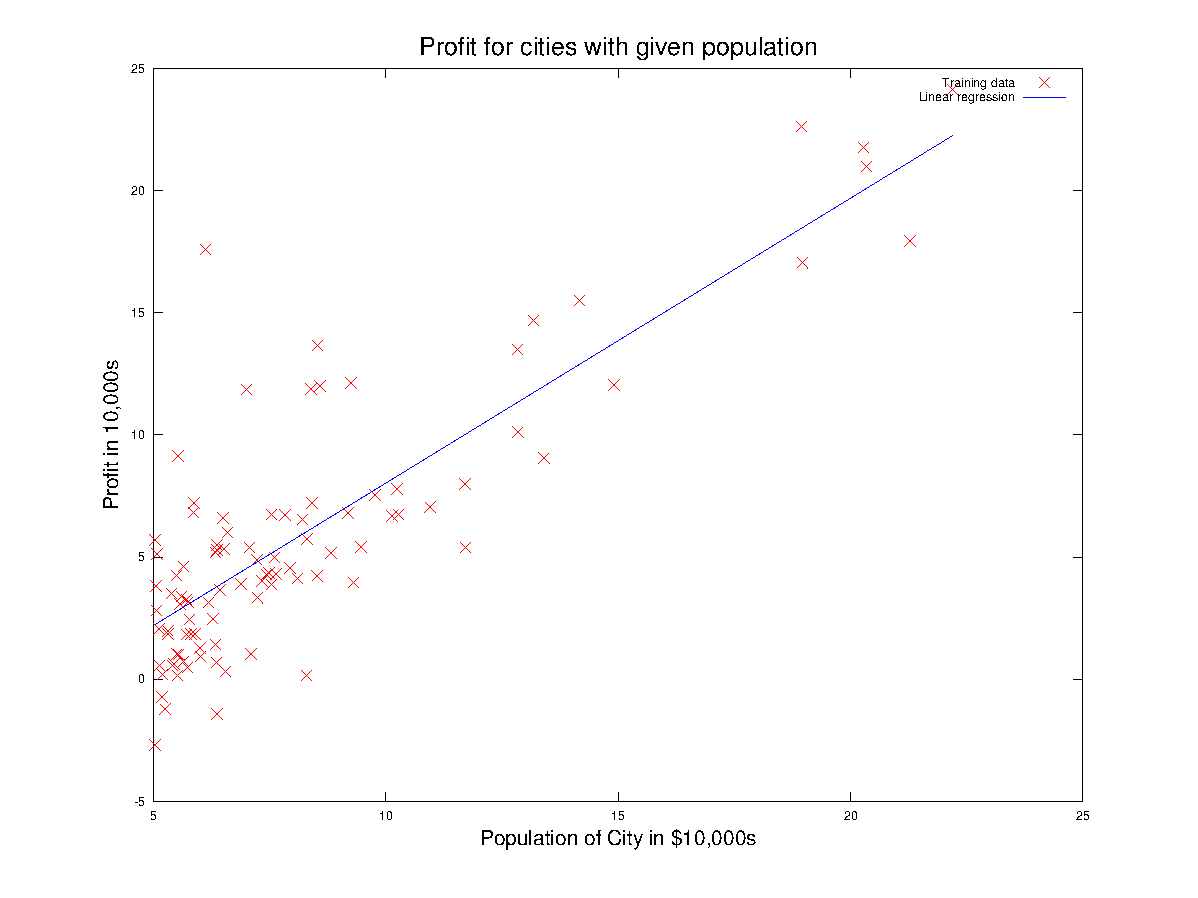
\includegraphics[width=.9\textwidth]{src/line_fit}
\caption{Линеарна регресија на тренинг множеството}
\label{fig:linear_fit}
\end{figure}

\subsubsection{Визуелизација на $J(\theta)$}
За подобро согледување на вредностите на функцијата на чинење $J(\theta)$ ги
исцртуваме нејзините вредност на 2-димензионален грид од вредностите
на $\theta_0$ и $\theta_1$.

Целта на овие графици е да покажат како $J(\theta)$ се менува со менувањето на
$\theta_0$ и $\theta_1$. Функцијата на чинење $J(\theta)$ е обликувана како
вдлабнат сад и има глобален минимум. Ова најубаво се воочува на површинскиот
график во 3Д. Минимумот е оптималната точка за $\theta_0$ и $\theta_1$, со што
алгоритмот gradient descent во секој чекор се доближува поблиску до оваа точка.


\begin{figure}[htbp]
        \begin{subfigure}[b]{0.5\textwidth}
                \centering
                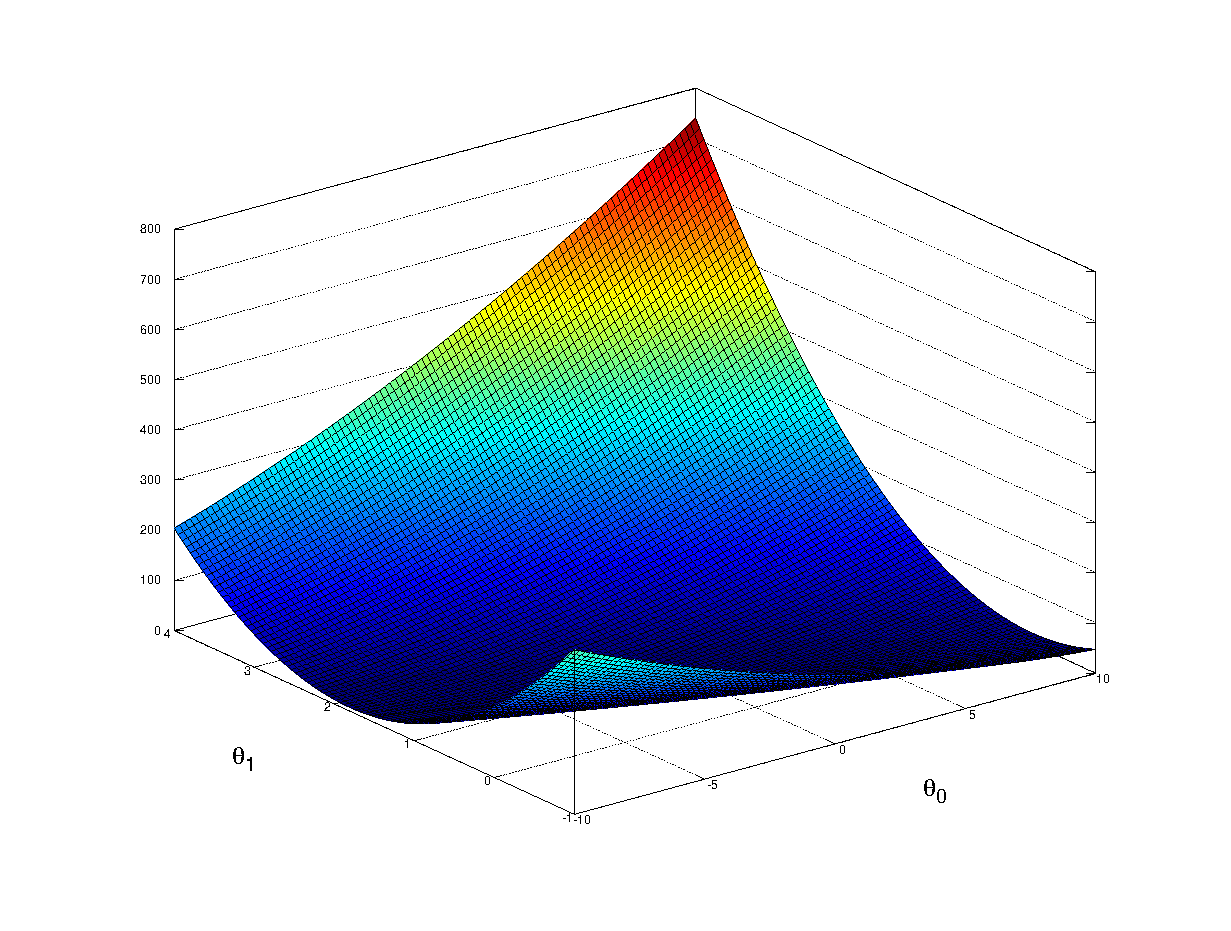
\includegraphics[width=\textwidth]{src/surface_plot}
                \caption{Површина}
                \label{fig:surface}
        \end{subfigure}%
        ~ 
        \begin{subfigure}[b]{0.5\textwidth}
                \centering
                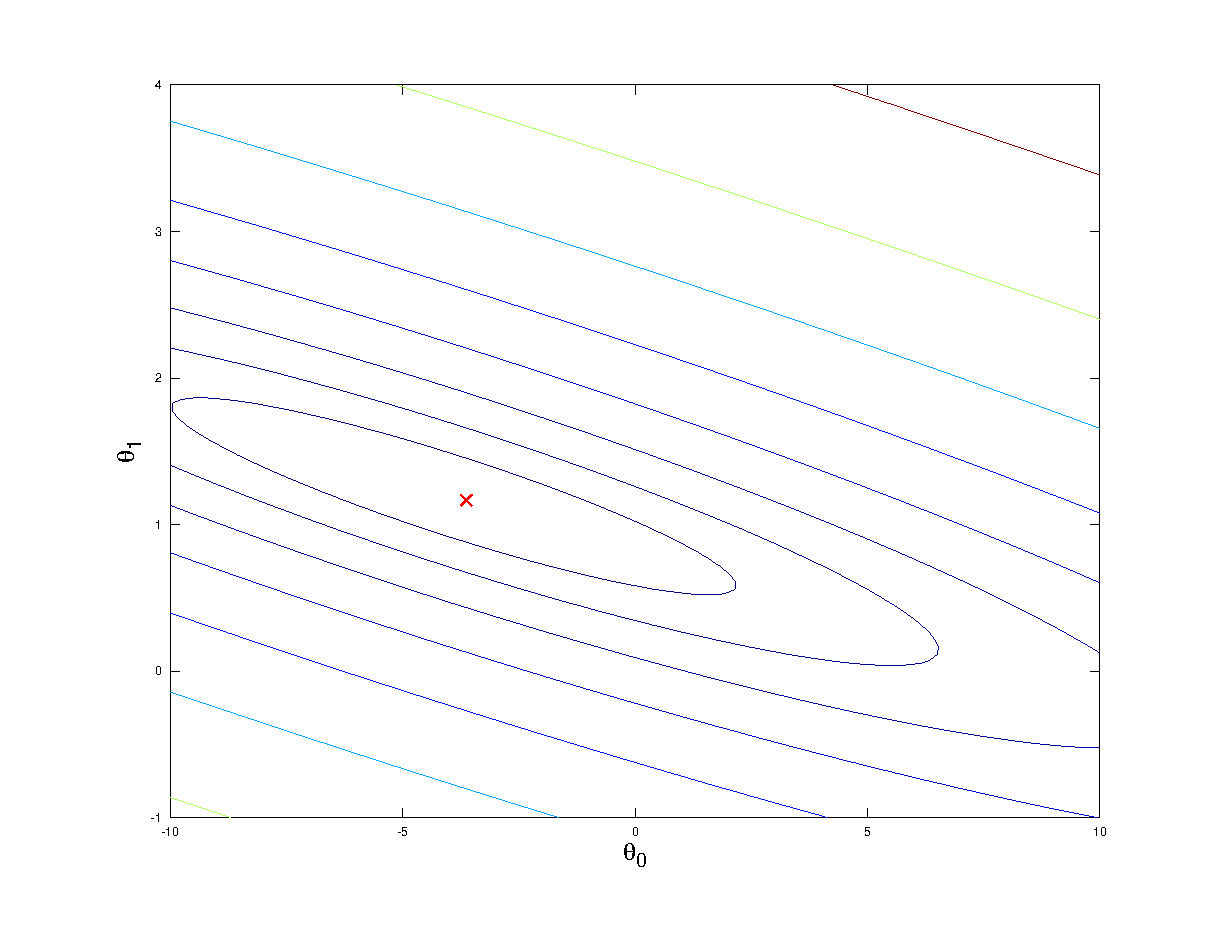
\includegraphics[width=\textwidth]{src/contour}
                \caption{Контура која го прикажува минимумот}
                \label{fig:contour}
        \end{subfigure}
        \caption{Функцијата на чинење $J(\theta)$}
        \label{fig:cost_function}
\end{figure}

\subsection{Линеарна регресија со повеќе променливи}

Со помош на линеарна регресија со повеќе променливи ќе ја предвидуваме цената на
куќите. Да претпоставиме дека продаваме куќа и сакаме да дознаеме која е
нејзината цена на пазарот. Еден начин да го дознаеме ова е да собереме
информации за цените на последно продадените куќи ид да изградиме модел на
цените на куќите.

Во датотеката houses\_prices.txt се содржи податочно множество со цените на
куќите во Портланд, Орегон. Првата колона е големината на куќата (во квадратни
стапки), втората колона е бројот на соби, а третата колона е цената на куќата.

\subsubsection{Нормализација на обележјата}

Помеѓу вредностите на некои обележја постојат многу големи разлики и тоа не е
добро за алгоритмите за машинско учење. Затоа кога постојат вакви огромни
разлики, вредностите на обележјата се нормализираат (скалираат) со што
алгоритмот gradient descent многу побрзо конвергира. 

Нормализацијата ја извршуваме со следните чекори:
\begin{itemize}
  \item Ја одземаме средната вредност од секое обележје во податочното
  множество,
  \item Ги скалираме (делиме) вредностите на обележјата со нивните соодветни
  стандардни девијации.
\end{itemize}

\lstinputlisting[firstline=8,lastline=16,caption=Нормализација
на обележјата]{src/featureNormalize.m}


\subsubsection{Gradient Descent}

\lstinputlisting[firstline=6,lastline=18,caption=Имплементација
на Gradient Descent за повеќе променливи]{src/gradientDescentMulti.m}


The vectorized version is efficient when you’re working with numerical
computing tools like Octave. If you are an expert with matrix operations,
you can prove to yourself that the two forms are equivalent.


Notice the changes in the convergence curves as the learning rate changes.
With a small learning rate, you should find that gradient descent takes a very
long time to converge to the optimal value. Conversely, with a large learning
rate, gradient descent might not converge or might even diverge!
Using the best learning rate that you found, run the ex1 multi.m script
to run gradient descent until convergence to find the final values of theta.
Next, use this value of THETA to predict the price of a house with 1650 square
feet and 3 bedrooms. You will use value later to check your implementation of the
normal equations. Don’t forget to normalize your features when you make
this prediction!
You do not need to submit any solutions for these optional (ungraded)
exercises.
3.3

Normal Equations
In the lecture videos, you learned that the closed-form solution to linear
regression is

Using this formula does not require any feature scaling, and you will get
an exact solution in one calculation: there is no “loop until convergence” like
in gradient descent.
Complete the code in normalEqn.m to use the formula above to calcu-
late THETA. Remember that while you don’t need to scale your features, we still
need to add a column of 1’s to the X matrix to have an intercept term (THETA0 ).
The code in ex1.m will add the column of 1’s to X for you.
You should now submit the normal equations function.
Optional (ungraded) exercise: Now, once you have found THETA using this
method, use it to make a price prediction for a 1650-square-foot house with
3 bedrooms. You should find that gives the same predicted price as the value
you obtained using the model fit with gradient descent (in Section 3.2.1)


\end{document}
